\lstset{
	basicstyle=\ttfamily\footnotesize,
	keywordstyle=\color{blue},
	stringstyle=\color{red},
	commentstyle=\color{gray},
	numbers=left,
	numberstyle=\tiny,
	stepnumber=1,
	numbersep=10pt,
	frame=single,
	breaklines=true,
	captionpos=b,
	tabsize=4,
	showspaces=false,
	showstringspaces=false,
	language=Python
}

\chapter{Hand Pose Feature Representation}
\begin{figure}[h!]
	\centering
	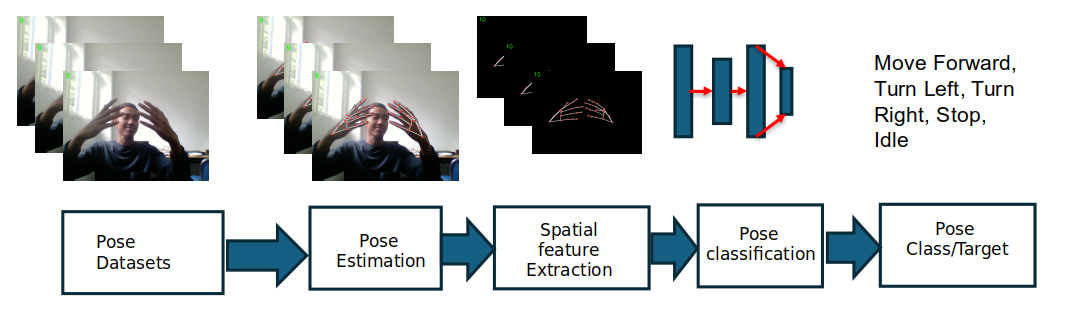
\includegraphics[width=\linewidth]{img/pose_pipeline} % Adjust the width or other parameters as needed
	\caption{Hand Recognition Pipeline}
	\label{fig:pose_pipeline} % Reference the figure in your text using \ref{fig:unique_label}
\end{figure}

\section{Geometric Feature}
Images captured from cameras exhibit a vast amount of variation. This is because images are spatial data, where each pixel represents a color at a specific coordinate. For pose classification, many images are required for training to account for differences in scale, position, and orientation of the hand in the images. The proposed geometric features were extracted from the coordinates of the hand joints. We used Google's MediaPipe Hands framework to track hand positions using joint coordinate landmarks. The framework provides three outputs: coordinates of landmark positions, a detection score that indicates the model's confidence in hand detection, and Handedness Classification, which identifies whether it is the left or right hand. 

\begin{figure}[h]
	\centering
	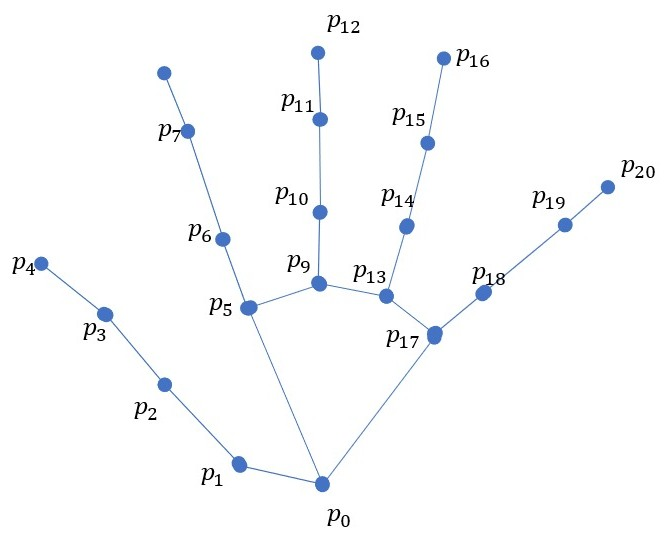
\includegraphics[width=\linewidth]{img/hand_feature} 
	\caption{The Feature on Hand Landmark}
	\label{fig:hand_feature} % Reference the figure in your text using \ref{fig:unique_label}
\end{figure}

The geometric features developed for this study were derived from the angles between the hand and joints. The selected hand joint angles are shown in Figure \ref{fig:hand_feature}.

\section{Normalized Geometric Feature}
In hand pose recognition, landmarks represent specific points on the hand, such as fingertips, joints, and the wrist. These landmarks are crucial geometric features used to describe the hand's pose. However, raw landmark coordinates can vary significantly depending on factors like hand position in the frame, distance from the camera, and individual hand size. To address this, normalization relative to landmark 0 (the wrist) and landmark 5 (the base of the index finger) ensures consistency and robustness. Normalization concerning landmark 0 and landmark 5 makes the model invariant to translation, scale, and individual hand size. By anchoring all landmarks to the wrist (landmark 0), the model ignores the absolute position of the hand in the image, focusing instead on its relative geometry \cite{10731943}. Scaling based on the distance between landmarks 0 and 5 compensates for variations in hand size or camera distance, ensuring that the features represent proportional relationships across individuals. This process reduces input variance, simplifies learning for the model, and ensures consistency in recognizing poses regardless of external conditions, such as hand position or size changes. The Figure \ref{fig:hand_feature_norm} represents the normalized geometric features.6
\begin{figure}[h]
	\centering
	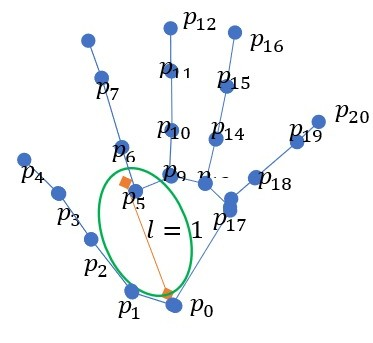
\includegraphics[width=0.7\linewidth]{img/hand_feature_normalized} 
	\caption{The Normalized Features on Hand Landmark}
	\label{fig:hand_feature_norm} % Reference the figure in your text using \ref{fig:unique_label}
\end{figure}

\section{Geometric Feature Joint}
In hand pose recognition \cite{9426433}, landmarks for the left and right hands are processed and combined to create a unified geometric representation. In the code, two arrays (\verb|left_hand_landmarks| and \verb|right_hand_landmarks|) are initialized to store the normalized landmarks for each hand. The function \verb|process_landmarks| normalizes the landmarks relative to the wrist (landmark 0) and scales them using the distance to landmark 5. This makes the landmarks invariant to translation, scale, and hand size.
When multiple hands are detected, the code uses the handedness attribute from Mediapipe to identify whether the landmarks belong to the left or right hand. The processed landmarks are stored in their respective arrays. After normalization, both sets of landmarks are flattened into 1D arrays and concatenated using \verb|np.concatenate|. This creates a single feature vector that includes both hands' landmarks.
Combining the landmarks into one representation allows the model to analyze interactions and spatial relationships between the hands. If only one hand is detected, the unused hand's array remains at zero, ensuring a consistent feature size for the model. This approach makes the representation robust and ready for gesture or sign language recognition tasks.